\documentclass[a4paper]{amsart}

\usepackage{amsmath}
\usepackage{graphicx}
\usepackage{subcaption}

\begin{document}

\section{Abbildungen}

\begin{figure}
    \caption{Kitty Warol}
    \begin{subfigure}[b]{0.3\textwidth}
        \caption{Erster Flug}
        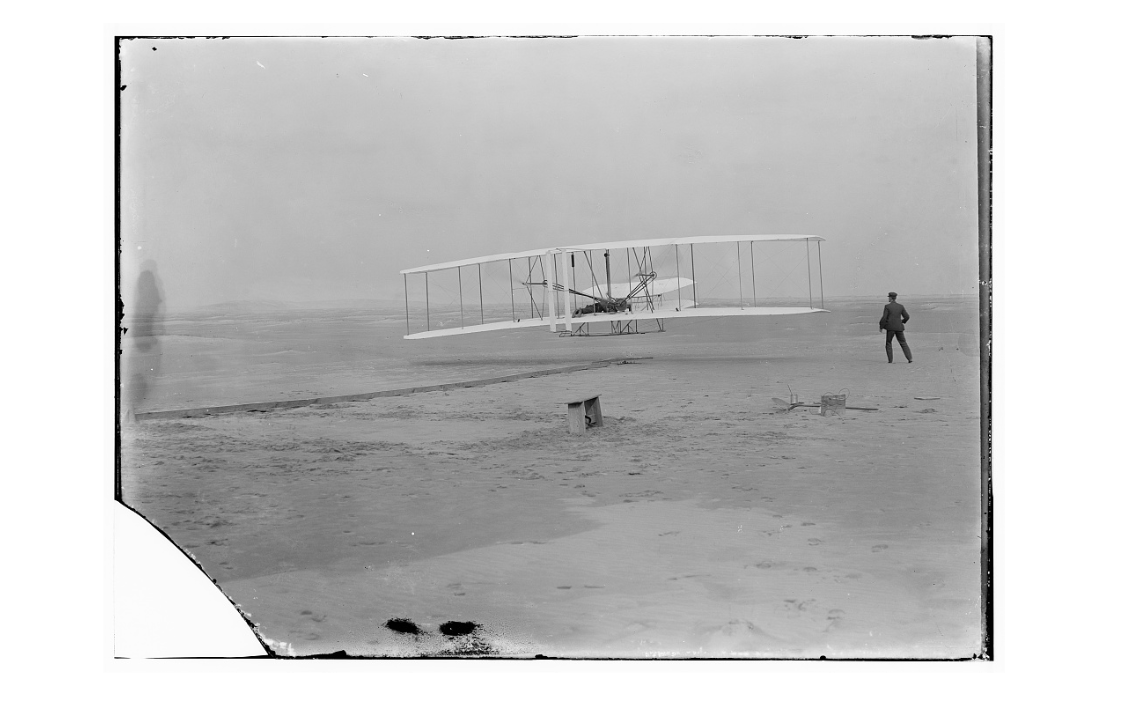
\includegraphics[width=\textwidth]{bild.png}
    \end{subfigure}
    \begin{subfigure}[b]{0.3\textwidth}
        \caption{Zweiter Flug}
        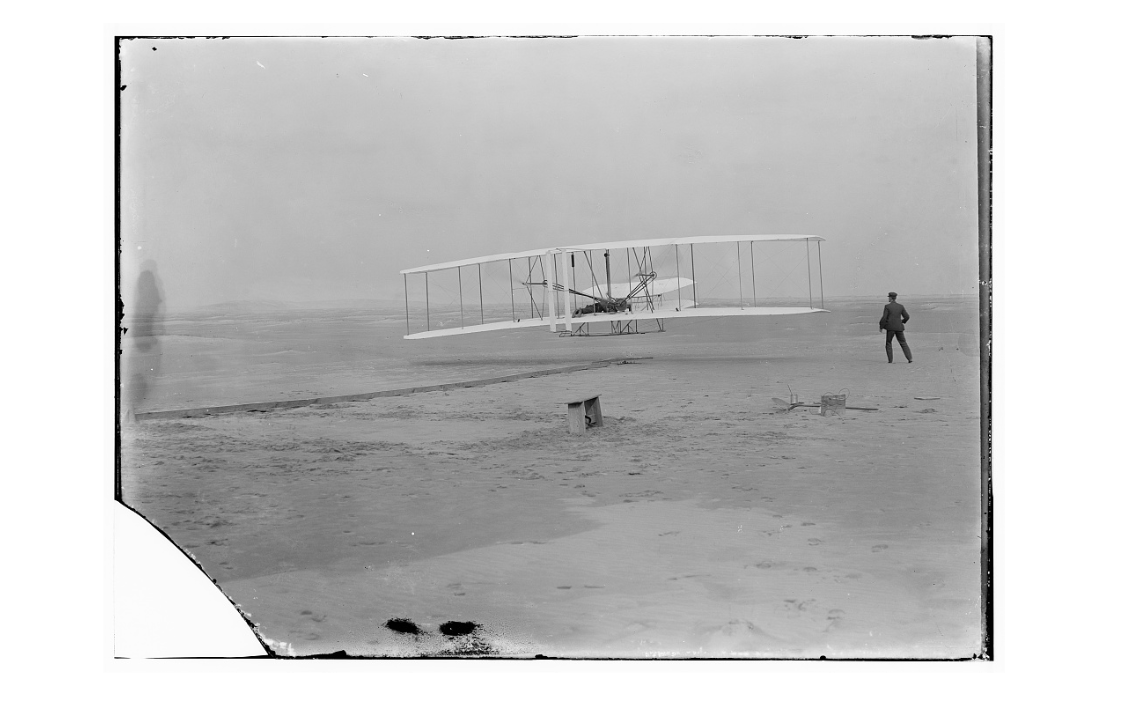
\includegraphics[width=\textwidth]{bild.png}
    \end{subfigure}
    \begin{subfigure}[b]{0.3\textwidth}
        \caption{Dritter Flug}
        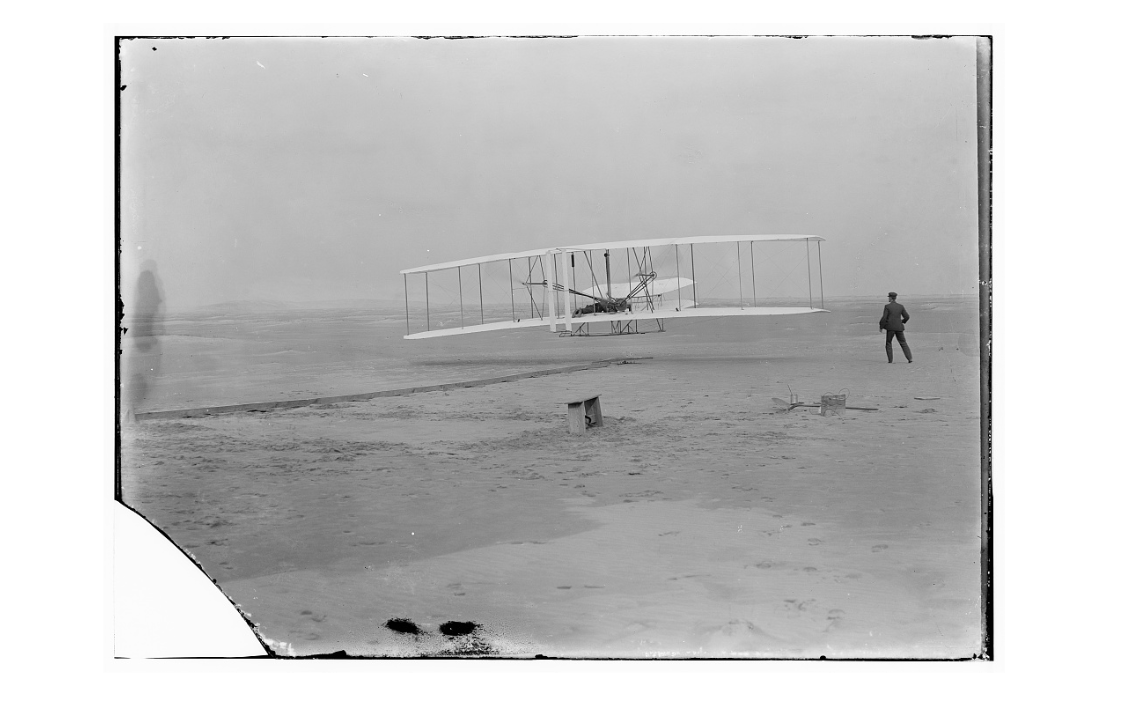
\includegraphics[width=\textwidth]{bild.png}
    \end{subfigure}
\end{figure}

Ohne:
\begin{figure}
    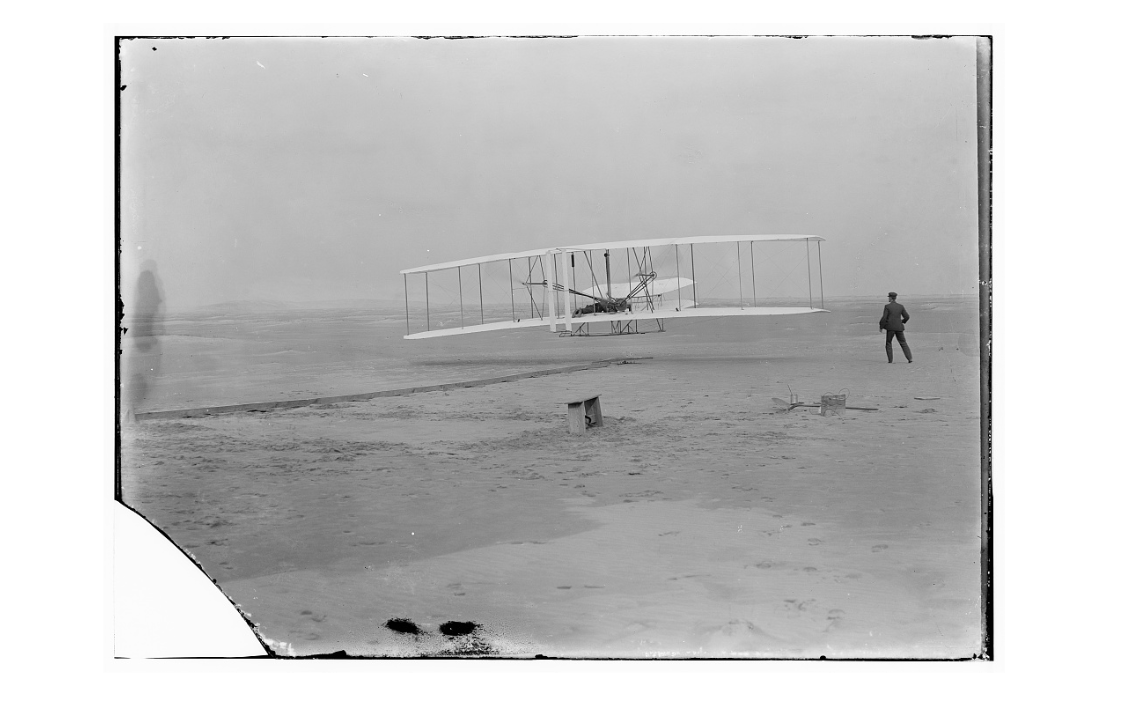
\includegraphics[width=\textwidth]{bild.png}
\end{figure}

Ups, floats.
\end{document}
